\documentclass[12pt]{scrartcl}
\usepackage{tikz}
\usepackage{amssymb}
\usetikzlibrary{positioning}
\usetikzlibrary{calc}
\usetikzlibrary{arrows,shapes,snakes,automata,petri}


\begin{document}
	
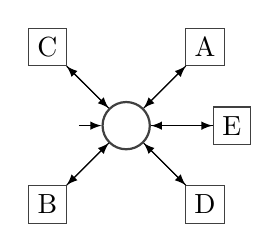
\begin{tikzpicture}
\tikzstyle{place} =[circle,thick,draw=black!75,minimum size=6mm]
\tikzstyle{transition} =[rectangle,draw=black!75,minimum size=4mm]
\node[place](init) at (0, 0) {};
\draw[draw,-latex]($(init)+(-0.6,0)$)--(init.west);

\node[transition](A) at ($(init)+(1,1)$){A};
\draw[draw,-latex] (init)--(A);
\draw[draw,-latex] (A)--(init);

\node[transition](B) at ($(init)+(-1,-1)$){B};
\draw[draw,-latex] (init)--(B);
\draw[draw,-latex] (B)--(init);

\node[transition](E) at ($(init)+(1.34,0)$){E};
\draw[draw,-latex] (init)--(E);
\draw[draw,-latex] (E)--(init);

\node[transition](C) at ($(init)+(-1,1)$){C};
\draw[draw,-latex] (init)--(C);
\draw[draw,-latex] (C)--(init);

\node[transition](D) at ($(init)+(1,-1)$){D};
\draw[draw,-latex] (init)--(D);
\draw[draw,-latex] (D)--(init);
\end{tikzpicture}
\end{document}